\documentclass[12pt, a4paper]{ctexart}

\usepackage{amsmath}
\usepackage{array}
\usepackage{appendix}
\usepackage{listings}
\usepackage{xcolor}
\usepackage{fontspec}
\usepackage{underscore}
\usepackage{graphicx}
\setmonofont{Consolas}
\lstset{
	breaklines=true,
	language = C++, 
	numbers=left,
	backgroundcolor=\color{red!0!green!25!blue!25},%代码块背景色为浅灰色
	rulesepcolor= \color{gray}, %代码块边框颜色
	numberstyle= \small,%行号字体
	frame=shadowbox%用方框框住代码块
	frame=single
}

\title{间断有限元第三次作业报告}
\author{九所 $\quad$ 韩若愚}
\date{2022.3.31}
\begin{document}
	\maketitle
	
	\section{题目}
	
	Considering the following Burgers equation
	
	\begin{equation}
	\begin{cases}
	& u_t + (]frac{u^2}{2})_x = 0,\\
	& u(x,0) = \frac{2}{3} + \frac{1}{3} \sin (\pi x),
	\end{cases}
	-1 \leq x \leq 1,
	\end{equation}
	with periodic boundary condition. Code up the DG scheme for $P^1$ and $P^2$, together with 2nd and 3rd order SSP RK method in time, respectively. Use uniform mesh is space.
	
	1. Take the final time at $T = 0.4$. Show error tables of the $L^2$ error, $L^\infty$ error and $|\int_{-1}^1 (u-u_h)\phi \, dx|$ with $\phi(x) = \cos(x)$.
	
	2. Take $T=1.5$. Show pictures of the exact solution and the numerical solution.
	
	\section{算法}
	
	\subsection{真解}
	
	由于方程是Burgers方程,所以真解$u$沿特征线$ \frac{dx}{dt} = u$不变。而特征线的斜率刚好是$u$,所以特征线是直线。于是真解为$u(x,t) = u(x- u(\xi,0)t,0)$,其中$\xi$为经过点$(x,t)$的特征线与$t=0$的交点。这个真解是隐式给出的,为了得到真解,需要得到经过点$(x,t)$的特征线的斜率$u(\xi,0)$。
	
	可以使用牛顿迭代法求$\xi$。因为$(x,t)$和$(\xi,0)$在同一条直线上,特征线方程$x = u(\xi,0)t+\xi$可改写为:
	$$
	f(\xi) := x - u_0(\xi) t - \xi = 0
	$$
	其中$u_0(x) = u(x,0)$。于是可以构造迭代公式:
	$$
	\xi^{(n+1)} = \xi^{(n)} - \frac{f(\xi^{(n)})}{f'(\xi^{(n)})}
	$$
	其中$\xi^{(n)}$表示第$n$个迭代值。
	
	\subsection{DG格式}
	
	首先对单元$[-1,1]$ 进行均匀剖分。假设将区间均匀剖分为$n$份,令:
	\begin{equation}
	0 = x_{\frac{1}{2}} < x_{\frac{3}{2}} < \dots < x_{n-\frac{1}{2}} < x_{n+\frac{1}{2}} = 1
	\end{equation}
	则第$j$个区间为:$ I_j = [x_{j- \frac{1}{2}}, x_{j + \frac{1}{2}}]$,每个区间的长度都为$h = \frac{2}{n}$。记$x_{j+1/2}^- = \lim_{x \in I_j, \, x \to x_{j+1/2}} \, x, \  x_{j+1/2}^+ = \lim_{x \in I_{j+1}, \, x \to x_{j+1/2}} \, x$。
	
	假设对固定的时间$t$,所求数值解$u_h(\cdot,t)$存在的空间为:$ V_h^k := \{ v : \  v|_{I_j} \in P^k(I_j), j = 1, \dots, n \}$,其中$k$为给定常数,$P^k(I_j)$为定义在$I_j$上的最高次项不超过$k$次的多项式空间。并假设检验函数$v \in V_h^k$,用$v$乘以方程两端并在$I_j$上积分。由于方程中通量函数$f(u) = \frac{u^2}{2}$是非线性的,在构造数值格式时需要要求当$k = 0$时,格式退化为一阶单调FD格式,于是空间离散后的半DG格式为:
	\begin{equation}
	\begin{split}
	& \int_{I_j} u_t v \, dx - \int_{I_j} (\frac{u^2}{2}) v_x \, dx\\
	& + \hat{f}_{j+1/2} v(x_{j+1/2}^-) - \hat{f}_{j-1/2} v(x_{j-1/2}^+) = 0, \quad j = 1,\dots,n
	\end{split}
	\label{1}
	\end{equation}
	其中$\hat{f}_{j+1/2}$是单调数值通量,保证在$k=0$时格式退化为1阶单调格式。$\hat{f}_{j+1/2} = \hat{f}(u_{j+1/2}^-, u_{j+1/2}^+)$。
	
	在$I_j$上取定一组$P^k(I_j)$的基底$\{ \phi_j^l \}_{l=0}^k$,则数值解$u_h$在$I_j$上表示为:$u_h(x,t) = \sum_{j=1}^n \sum_{l=0}^k \, u_j^l(t) \, \phi_j^l(x)$,求解$u_h$即求解系数$u_j^l, \, j=1, \dots, n, \, l=0, \dots, k$。令检验函数$v = \phi_j^m, \, m=0, \dots, k$,则方程组(\ref{1})变为:
	\begin{equation}
	\begin{split}
	& \sum_{l=0}^k \int_{I_j} \phi_j^l \phi_j^m \, dx \, u_j^l - \frac{1}{2}\sum_{p,q=0}^k \int_{I_j} \phi_j^p \phi_j^q (\phi_j^m)_x \, dx \, u_j^p u_j^q \\
	& + \hat{f}(\sum_{l=0}^k u_j^l \phi_j^l(x_{j+1/2}),u_{j+1/2}^+) \phi_j^m(x_{j+1/2})\\
	& - \hat{f}(u_{j-1/2}^-, \sum_{l=0}^k u_j^l \phi_j^l(x_{j-1/2} )) \phi_j^m(x_{j-1/2}) = 0, \quad j = 1, \dots,n
	\end{split}
	\label{2}
	\end{equation}
	这是关于向量$\textbf{u}_j = (u_j^0,\dots, u_j^k)$的$m$维方程组。
	
	为便于求解,假设参考单元$I = [-1,1]$,对每个单元$I_j$都有一个到$I$的微分同胚$\Phi_j : I_j \to I$,$ \xi := \Phi_j(x) = \frac{2}{h} (x - x_{j-1/2}) - 1$。在参考单元上取定一组$P^k(I)$的基底$\{\phi^l\}_{l=0}^k$,则由$\Phi_j$将$\phi^l$拉回到$I_j$上得到的函数组$\{(\Phi_j^{-1})^* \phi^l\}$也是$P^k(I_j)$的基底,不妨就设为$\{\phi_j^l\}$。于是每个单元$I_j$上的计算都可以在$I$上进行,方程组(\ref{2})变为:
	\begin{equation}
	\begin{split}
	&  \frac{h}{2} \sum_{l=0}^k \int_I \phi^l \phi^m \, d\xi \, u_j^l -\frac{1}{2} \sum_{p,q=0}^k \int_I \phi^p \phi^q (\phi^m)_\xi \, d\xi \, u_j^p u_j^q \\
	& + \hat{f}(\sum_{l=0}^k u_j^l \phi^l(1),u_{j+1/2}^+) \phi^m(1)\\
	& - \hat{f}(u_{j-1/2}^-, \sum_{l=0}^k u_j^l \phi^l(-1)) \phi^m(-1) = 0, \quad j = 1, \dots,n
	\end{split}
	\label{3}
	\end{equation}
	其中$u_{j+1/2}^+ = \sum_{l=0}^k u_{j+1}^l \phi^l(-1)$,$u_{j-1/2}^- = \sum_{l=0}^k u_{j-1}^l \phi^l(1)$,$j$为循环指标。
	
	(\ref{3})可以写为向量形式:
	$$
	\frac{h}{2} A \frac{d}{dt} \textbf{u}_j = \frac{1}{2} \textbf{u}_j B \textbf{u}_j - C_j
	$$
	\begin{equation}
	\frac{d}{dt} \textbf{u}_j = \frac{2}{h} A^{-1} (\frac{1}{2} \textbf{u}_j B \textbf{u}_j - C_j) := L_j(\textbf{u}_j)
	\label{4}
	\end{equation}
	其中$A$为$(k+1) \times (k+1)$维矩阵,$A_{ml} = \int_I phi^l \phi^m \, d\xi$,$B$为三阶张量,$B = \int_I \phi^p \phi^q (\phi^m)_\xi \, d\xi \, \omega^p \otimes \omega^q \otimes \omega^m$,其中$\omega^i$是取定的余切标架场,在本例中即自然标架场的对偶标架场。$C_j$为$m$维向量,$C_{j,m} = \hat{f}(\sum_{l=0}^k u_j^l \phi^l(1),u_{j+1/2}^+) \phi^m(1)- \hat{f}(u_{j-1/2}^-, \sum_{l=0}^k u_j^l \phi^l(-1)) \phi^m(-1)$。于是(\ref{4})可以用R-K法求解。求解前还需要得到$\textbf{u}_j$的初值,对初值$u(x,0)$做到$P^k(I_j)$上的$L^2$投影:对任意$j=1,2,\dots,n, \  m = 0,1,\dots,k$,有
	$$
	\int_{I_j} u(x,0) \phi_j^m(x) \, dx  = \int_{I_j} \sum_{l=0}^k u_j^l(0) \phi_j^l(x) \phi_j^m(x) \, dx.
	$$
	
	SSPRK(2,2)和SSPRK(3,3)格式分别如下:
	\begin{align*}
	&SSPRK(2,2):\\
	& \quad u^{(0)} = u^n\\
	& \quad u^{(1)} = u^{(0)} + \Delta t F(u^{(0)})\\
	& \quad u^{n+1} = \frac{1}{2} u^{(0)} + \frac{1}{2} u^{(1)} + \frac{1}{2} \Delta t F(u^{(1)})\\
	&\\
	&SSPRK(3,3):\\
	& \quad u^{(0)} = u^n\\
	& \quad u^{(1)} = u^{(0)} + \Delta t F(u^{(0)})\\
	& \quad u^{(2)} = \frac{3}{4} u^{(0)} + \frac{1}{4} u^{(1)} + \frac{1}{4} \Delta t F(u^{(1)}) \\
	& \quad u^{n+1} = \frac{1}{3} u^{(0)} + \frac{2}{3} u^{(2)} + \frac{2}{3} \Delta t F(u^{(2)})
	\end{align*}
	
	同时为保证稳定性,对时间步长$\Delta t$的选取还要满足CFL条件。
	
	\section{计算结果}
	为了方便计算,取$P^k(I)$上的基函数为Legendre函数。数值通量选为Lax-Fridrichs通量:
	$$
	\hat{f}(u^-,u^+) = \frac{1}{2}(f(u^-) + f(u^+) - \alpha (u^- - u^+))
	$$
	其中$\alpha = \max_{u|_{I_j}} |f'(u) |$。为了满足CFL条件并观察到超收敛性,将时间步长$\Delta t$取为$h^2$。算法使用C++实现。
	
	在终止时刻$t=0.4$时计算真解与数值解的$L^2$范数、$L^\infty$范数误差和误差$|
	int_{-1}^1 (u-u_h)\cos(x) \, dx|$。$P^1,P^2$元的误差表如下(保留三位小数):
	\begin{table}[htbp]
		\centering
		\caption{$P^1$}
		\begin{tabular}{| p{20pt}<{\centering} | p{50pt}<{\centering} | p{40pt}<{\centering} || p{50pt}<{\centering} | p{40pt}<{\centering}|| p{50pt}<{\centering} | p{40pt}<{\centering}|}
			\hline
			n & $L^2$ error & order & $L^\infty$error & order & $H^{-k}$error & order\\
			\hline
			10 & 1.005e-2 & & 2.670e-2 &  & 1.297e-4 & \\
			\hline
			20 & 2.678e-3 & 1.908 & 7.895e-3 & 1.758 & 2.410e-5 & 2.428 \\
			\hline
			40 & 6.941e-4 & 1.948 & 2.126e-3 & 1.893 & 3.410e-6 & 2.821\\
			\hline
			80 & 1.765e-4 & 1.975 & 5.537e-4 & 1.941 & 4.464e-7 & 2.933\\
			\hline
			160 & 4.448e-5 & 1.988 & 1.413e-4 & 1.970 & 5.694e-8 & 2.971\\
			\hline
			320 & 1.116e-5 & 1.995 & 3.566e-5 & 1.986 & 7.238e-9 & 2.976\\
			\hline
		\end{tabular}
	\end{table}

	\begin{table}[htbp]
	\centering
	\caption{$P^2$}
	\begin{tabular}{| p{20pt}<{\centering} | p{50pt}<{\centering} | p{40pt}<{\centering} || p{50pt}<{\centering} | p{40pt}<{\centering}|| p{50pt}<{\centering} | p{40pt}<{\centering}|}
		\hline
		n & $L^2$ error & order & $L^\infty$error & order & $H^{-k}$error & order\\
		\hline
		10 & 1.091e-3 & & 4.615e-3 &  & 6.730e-6 & \\
		\hline
		20 & 1.472e-4 & 2.900 & 7.674e-4 & 2.588 & 1.481e-7 & 5.506 \\
		\hline
		40 & 1.914e-5 & 2.943 & 1.027e-4 & 2.902 & 3.382e-9 & 5.453 \\
		\hline
		80 & 2.442e-6 & 2.970 & 1.383e-5 & 2.893 & 1.655e-10 & 4.353\\
		\hline
		160 & 3.082e-7 & 2.986 & 1.759e-6 & 2.975 & 4.036e-11 & 2.036\\
		\hline
		320 & 3.896e-8 & 2.984 & 2.342e-7 & 2.909 & 5.900e-11 & -0.548\\
		\hline
	\end{tabular}
	\end{table}
	
	当终止时刻$T = 1.5$时,在$x=0$处特征线会相交,出现激波。当$n=80$时得到的真解$u$和数值解$u_h$的图像如下:
	\begin{figure}[htbp]
		\centering
		\caption{$P^1$}
		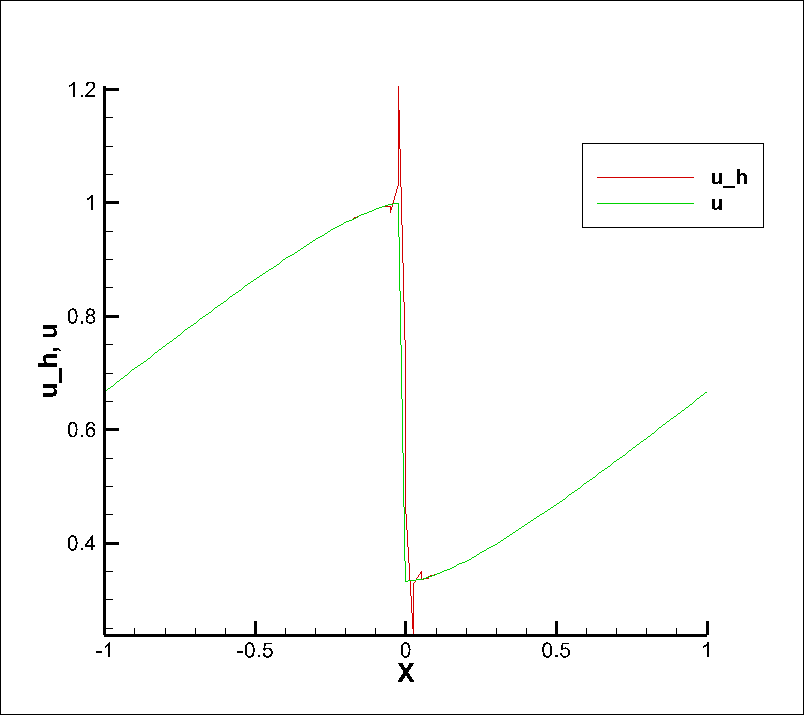
\includegraphics[width=15cm]{P1.png}
	\end{figure}
	\begin{figure}[htbp]
		\centering
		\caption{$P^2$}
		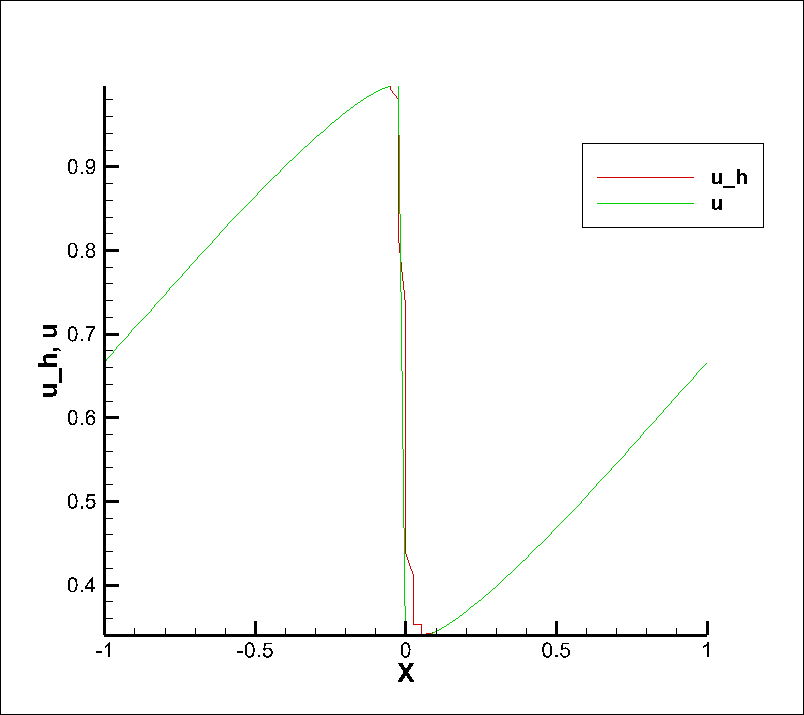
\includegraphics[width=15cm]{1.5.png}
	\end{figure}

	\newpage
	\section{分析}
	
	可以看到当$k$分别等于1,2时,$L^2$和$L^\infty$误差分别在2,3附近。当$k=1$时,负模误差接近3,出现了超收敛现象。而当$k=2$时负模的误差一直在减小,在$n\leq80$时存在超收敛现象,但是$n>80$后误差基本没有改变反而增长了。如果将$\Delta t$调小,情况也没有太大改变。我的程序使用的是双精度浮点数,在C++中应该能达到$10^{308}$数量级,按道理应该不会出现这种情况的,但是到目前为止我还没有想明白问题在哪里。
	
	而当$T=1.5$时,计算结果在$k=0$时在$=0$处出现了明显振荡,而当$k=1$时震荡并不是十分明显。
	
	\section{源代码}
	
	本次报告程序使用C++编译。
	
	\appendix
	
	\begin{lstlisting}
	#include <iostream>
	#include <cmath>
	#include <fstream>
	using namespace std;
	
	//先定义一些全局的变量
	const int n = 80;   //划分单元个数
	const int k = 1;    //多项式最高次项次数
	const double h = (double) 2/n;    //空间步长
	const double dt = (double) h * h;    //时间步长
	const double pi = 3.1415926;
	
	double p[n+1];  //节点位置,p_j = j * h = x_{j+1/2}, j =0,1, ..., n
	//存储不变的系数矩阵
	
	const double Legendre[5] = {-0.9061798459,-0.5384693101,0.,
	0.5384693101,0.9061798459};
	const double LegendreCo[5] = {0.2369268851,0.4786286705,0.5688888889,
	0.4786286705,0.2369268851};
	
	//*************函数声明*************//
	double u_0(double y);   //初值
	double u_exact(double y, double t);   //真解
	double f(double y); //通量函数
	double phi(int l, double y);    //参考单元基函数
	double** initial();   //计算初始时刻u_j
	double flux(double ul, double ur);  //数值通量计算
	double** L(double** ut);   //用于计算RK的函数,u_t= F(u)
	double** RK22(double** un);    //2步二阶RK
	double** RK33(double** un);
	double** RK(int k, double** un);
	//************声明完毕**************//
	
	int main()
	{
	int i, j, l;
	double t, temp1, temp2, norm1, norm2, norm3, xi;
	double T = 1.5;
	double** u1 = new double* [n];
	double** u2 = new double* [n];
	for (i=0; i<n; i++)
	{
	u1[i] = new double [k+1];
	u2[i] = new double [k+1];
	}
	for (j=0; j<=n; j++)
	{
	p[j] = j * h - 1;
	}
	
	
	u1 = initial();
	t = 0;
	while(t<T - 1e-10)
	{
	
	t = t + dt;
	u2 = RK(k,u1);
	
	u1 = u2;
	cout<<t<<endl;
	}
	
	//*
	norm1 = 0;
	norm2 = 0;
	norm3 = 0;
	for (j=1; j<=n; j++)
	{
	
	for (i=0; i<5; i++)
	{
	xi = Legendre[i];
	temp1 = 0;
	for (l=0; l<=k; l++)
	{
	temp1 = temp1 + u1[j-1][l] * phi(l,xi);
	}
	
	temp2 = h * (xi + 1) / 2. + p[j-1];
	temp1 = u_exact(temp2,T) - temp1;
	
	if (abs(temp1) > norm2)
	{
	norm2 = abs(temp1);
	}
	
	norm3 = norm3 + LegendreCo[i] * temp1 * cos(temp2);
	
	temp1 = temp1 * temp1;
	norm1 = norm1 + LegendreCo[i] * temp1;
	}
	
	}
	norm1 = norm1 * h / 2.;
	norm1 = sqrt(norm1);
	norm3 = norm3 * h / 2.;
	norm3 = abs(norm3);
	cout<<"L2="<<norm1<<endl<<"Linf="<<norm2<<endl<<"Lphi="<<norm3<<endl;//*/
	
	{
	const char* fn = "DGLecture\\homework3\\output.plt";
	remove(fn);
	fstream f, f1;
	f.open(fn, ios::out | ios :: app);
	f<<"VARIABLES="<<"X"<<","<<"u_h"<<","<<"u"<<endl;
	for (j=1; j<=n; j++)
	{
	temp1 = 0;
	temp2 = 0;
	for (l=0; l<=k; l++)
	{
	temp1 = temp1 + u1[j-1][l] * phi(l,-1);
	temp2 = temp2 + u1[j-1][l] * phi(l,1);
	}
	f<<"\t"<<p[j-1]<<"\t"<<temp1<<"\t"<<u_exact(p[j-1],T)<<endl;
	f<<"\t"<<p[j]<<"\t"<<temp2<<"\t"<<u_exact(p[j],T)<<endl;
	}
	f.close();
	}
	
	for (i=0; i<n; i++)
	{
	delete[] u1[i];
	delete[] u2[i];
	}
	delete[] u1;
	delete[] u2;
	
	system("pause");
	}
	
	double u_0(double y)
	{
	return sin(pi*y) / 3.0 + 2.0 / 3.0 ;
	}
	
	double u_exact(double y, double t)
	{
	int time=1;
	double ans, xi1=0, xi2=0.1;
	double e = 1e-6;
	
	//if (t==1.5)  //1.5时刻发生激波,单独算
	{
	if (y < -1+2*t/3.0)
	{
	y = y+2;
	}
	}
	
	while(abs(xi1 - xi2)>e)
	{
	xi1 = xi2;
	xi2 = xi1 + ( y - u_0(xi1) * t - xi1 ) / (t * pi * cos(pi*xi1)/3.0 + 1);
	time++;
	if (time > 10000)
	{
	cout<<"error"<<endl;
	cout<<y<<endl;
	break;
	}
	}
	ans = u_0(xi2);
	
	return ans;
	}
	
	double f(double y)
	{
	return y * y /2;
	}
	
	double phi(int l, double y)
	{
	if (l==0)
	{
	return 1;
	}
	else if (l == 1)
	{
	return y;
	}
	else if (l == 2)
	{
	return (3*y*y - 1)/2;
	}
	else{
	return 0;
	}
	}
	
	double** initial()
	{
	double ans, temp;
	int j, l, m;
	double** ut = new double* [n];
	double* Bt = new double [n];
	for (j=0; j<n; j++)
	{
	ut[j] = new double [k+1];
	}
	
	for (j=1; j<=n; j++)
	{
	for (m=0; m<=k; m++)
	{
	ans = 0;
	for (l=0; l<5; l++)
	{
	temp = h * (Legendre[l] + 1)/2 + p[j-1];
	ans = ans + LegendreCo[l] * u_0(temp) * phi(m,Legendre[l]);
	}
	ans = ans / 2;
	Bt[m] = ans;
	}
	
	double A[3][3] = {{1,0,0},{0,3,0},{0,0,5}};
	for (m=0; m<=k ;m++)
	{
	ut[j-1][m] = 0;
	for (l=0; l<=k; l++)
	{
	ut[j-1][m] = ut[j-1][m] + A[m][l] * Bt[l];
	}
	}
	
	}
	
	delete[] Bt;
	
	return ut;
	}
	
	double flux(double ul, double ur)
	{
	double ans, alpha;
	int i, l;
	if ( ul <= ur)
	{
	//ans = f(ul);  //Godnov
	alpha = ur; //Lax-Friedrichs
	}
	else{
	//ans = f(ul);
	alpha = ul;
	}
	
	ans = f(ul) + f(ur) - alpha * (ur - ul);
	ans = ans * 0.5;
	
	return ans;
	}
	
	double** L(double** ut)
	{
	int i, j, l, m, p, q;
	double ul, ur;
	double** ans = new double* [n];
	for (i=0; i<n; i++)
	{
	ans[i] = new double [k+1];
	}
	
	double A[3] = {1,3,5};
	double B[3][3][3] = {{{0,0,0},{0,0,0},{0,0,0}}, {{2,0,0},{0,2.0/3.0,0},{0,0,2.0/5.0}}, {{0,2,0},{2,0,4.0/5.0},{0,4.0/5.0,0}}};
	
	
	for (j=1; j<=n; j++)
	{
	for (m=0; m<=k; m++)
	{
	ans[j-1][m] = 0;
	
	for (p=0; p<=k; p++)
	{
	for (q=0; q<=k; q++)
	{
	ans[j-1][m] = ans[j-1][m] + ut[j-1][p] * B[m][p][q] * ut[j-1][q];
	}
	}
	ans[j-1][m] = ans[j-1][m] / 2;
	
	//计算第一个数值通量
	{
	ul = 0;
	ur = 0;
	q = j;
	if (q == n)
	{
	q = 0;
	}
	for (l=0; l<=k; l++)
	{
	ul = ul + ut[j-1][l] * phi(l,1);
	ur = ur + ut[q][l] * phi(l,-1);
	}
	ans[j-1][m] = ans[j-1][m] - flux(ul,ur) * phi(m,1);
	
	}
	
	//计算第二个数值通量
	{
	ul = 0;
	ur = 0;
	
	p = j-2;
	if ( p == -1)
	{
	p = n-1;
	}
	for (l=0; l<=k; l++)
	{
	ul = ul + ut[p][l] * phi(l,1);
	ur = ur + ut[j-1][l] * phi(l,-1);
	}
	ans[j-1][m] = ans[j-1][m] + flux(ul,ur) * phi(m,-1);
	}
	
	ans[j-1][m] = ans[j-1][m] * A[m] / h;
	}
	}
	
	return ans;
	}
	
	double** RK22(double** un)
	{
	int j,l,m;
	double ul;
	double** ans = new double* [n];
	for (j=0; j<n; j++)
	{
	ans[j] = new double [k+1];
	}
	double** u0 = new double* [n];
	double** u1 = new double* [n];
	double** u2 = new double* [n];
	
	for (j=0; j<n; j++)
	{
	u0[j] = new double [k+1];
	u1[j] = new double [k+1];
	u2[j] = new double [k+1];
	}
	
	for (j=1; j<=n; j++)
	{
	for (l=0; l<=k; l++)
	{
	u0[j-1][l] = un[j-1][l];
	}
	}
	
	u1 = L(u0);
	for (j=1; j<=n; j++)
	{
	for (l=0; l<=k; l++)
	{
	u1[j-1][l] = u1[j-1][l] * dt  + u0[j-1][l];
	}
	}
	
	
	u2 = L(u1);
	for (j=1; j<=n;j++)
	{
	for (l=0; l<=k; l++)
	{
	u2[j-1][l] = u0[j-1][l] * 0.5 + u1[j-1][l] * 0.5 + u2[j-1][l] * 0.5 * dt;
	ans[j-1][l] = u2[j-1][l];
	}
	}
	
	
	delete[] u0;
	delete[] u1;
	delete[] u2;
	
	return ans;
	}
	
	double** RK33(double** un)
	{
	int j,l,m;
	double ul;
	double** ans = new double* [n];
	for (j=0; j<n; j++)
	{
	ans[j] = new double [k+1];
	}
	double** u0 = new double* [n];
	double** u1 = new double* [n];
	double** u2 = new double* [n];
	double** u3 = new double* [n];
	
	for (j=0; j<n; j++)
	{
	u0[j] = new double [k+1];
	u1[j] = new double [k+1];
	u2[j] = new double [k+1];
	u3[j] = new double [k+1];
	}
	
	for (j=1; j<=n; j++)
	{
	for (l=0; l<=k; l++)
	{
	u0[j-1][l] = un[j-1][l];
	}
	}
	
	u1 = L(u0);
	for (j=1; j<=n; j++)
	{
	for (l=0; l<=k; l++)
	{
	u1[j-1][l] = u1[j-1][l] * dt  + u0[j-1][l];
	}
	}
	
	
	u2 = L(u1);
	for (j=1; j<=n;j++)
	{
	for (l=0; l<=k; l++)
	{
	u2[j-1][l] = u0[j-1][l] * 3 / 4 + u1[j-1][l] /4 + u2[j-1][l] * dt / 4;
	}
	}
	
	u3 = L(u2);
	for (j=1; j<=n; j++)
	{
	for (l=0; l<=k; l++)
	{
	u3[j-1][l] = u0[j-1][l] / 3 + 2 * u2[j-1][l] / 3 + 2 * dt * u3[j-1][l] /3;
	ans[j-1][l] = u3[j-1][l];
	}
	}
	
	
	delete[] u0;
	delete[] u1;
	delete[] u2;
	delete[] u3;
	
	return ans;
	}
	
	double** RK(int k, double** un)
	{
	double** u2;
	if ( k == 1 )
	{
	u2 = RK22(un);
	}
	else if (k == 2)
	{
	u2 = RK33(un);
	}
	else{
	;
	}
	
	return u2;
	}
	\end{lstlisting}
		
	
	
\end{document}